% Template for PLoS
% Version 3.5 March 2018
%
% % % % % % % % % % % % % % % % % % % % % %
%
% -- IMPORTANT NOTE
%
% This template contains comments intended
% to minimize problems and delays during our production
% process. Please follow the template instructions
% whenever possible.
%
% % % % % % % % % % % % % % % % % % % % % % %
%
% Once your paper is accepted for publication,
% PLEASE REMOVE ALL TRACKED CHANGES in this file
% and leave only the final text of your manuscript.
% PLOS recommends the use of latexdiff to track changes during review, as this will help to maintain a clean tex file.
% Visit https://www.ctan.org/pkg/latexdiff?lang=en for info or contact us at latex@plos.org.
%
%
% There are no restrictions on package use within the LaTeX files except that
% no packages listed in the template may be deleted.
%
% Please do not include colors or graphics in the text.
%
% The manuscript LaTeX source should be contained within a single file (do not use \input, \externaldocument, or similar commands).
%
% % % % % % % % % % % % % % % % % % % % % % %
%
% -- FIGURES AND TABLES
%
% Please include tables/figure captions directly after the paragraph where they are first cited in the text.
%
% DO NOT INCLUDE GRAPHICS IN YOUR MANUSCRIPT
% - Figures should be uploaded separately from your manuscript file.
% - Figures generated using LaTeX should be extracted and removed from the PDF before submission.
% - Figures containing multiple panels/subfigures must be combined into one image file before submission.
% For figure citations, please use "Fig" instead of "Figure".
% See http://journals.plos.org/plosone/s/figures for PLOS figure guidelines.
%
% Tables should be cell-based and may not contain:
% - spacing/line breaks within cells to alter layout or alignment
% - do not nest tabular environments (no tabular environments within tabular environments)
% - no graphics or colored text (cell background color/shading OK)
% See http://journals.plos.org/plosone/s/tables for table guidelines.
%
% For tables that exceed the width of the text column, use the adjustwidth environment as illustrated in the example table in text below.
%
% % % % % % % % % % % % % % % % % % % % % % % %
%
% -- EQUATIONS, MATH SYMBOLS, SUBSCRIPTS, AND SUPERSCRIPTS
%
% IMPORTANT
% Below are a few tips to help format your equations and other special characters according to our specifications. For more tips to help reduce the possibility of formatting errors during conversion, please see our LaTeX guidelines at http://journals.plos.org/plosone/s/latex
%
% For inline equations, please be sure to include all portions of an equation in the math environment.  For example, x$^2$ is incorrect; this should be formatted as $x^2$ (or $\mathrm{x}^2$ if the romanized font is desired).
%
% Do not include text that is not math in the math environment. For example, CO2 should be written as CO\textsubscript{2} instead of CO$_2$.
%
% Please add line breaks to long display equations when possible in order to fit size of the column.
%
% For inline equations, please do not include punctuation (commas, etc) within the math environment unless this is part of the equation.
%
% When adding superscript or subscripts outside of brackets/braces, please group using {}.  For example, change "[U(D,E,\gamma)]^2" to "{[U(D,E,\gamma)]}^2".
%
% Do not use \cal for caligraphic font.  Instead, use \mathcal{}
%
% % % % % % % % % % % % % % % % % % % % % % % %
%
% Please contact latex@plos.org with any questions.
%
% % % % % % % % % % % % % % % % % % % % % % % %

\documentclass[10pt,letterpaper]{article}
\usepackage[top=0.85in,left=2.75in,footskip=0.75in]{geometry}

% amsmath and amssymb packages, useful for mathematical formulas and symbols
\usepackage{amsmath,amssymb}

% Use adjustwidth environment to exceed column width (see example table in text)
\usepackage{changepage}

% Use Unicode characters when possible
\usepackage[utf8x]{inputenc}

% textcomp package and marvosym package for additional characters
\usepackage{textcomp,marvosym}

% cite package, to clean up citations in the main text. Do not remove.
\usepackage{cite}

% Use nameref to cite supporting information files (see Supporting Information section for more info)
\usepackage{nameref,hyperref}

% line numbers
\usepackage[right]{lineno}

% ligatures disabled
\usepackage{microtype}
\DisableLigatures[f]{encoding = *, family = * }

% color can be used to apply background shading to table cells only
\usepackage[table]{xcolor}

% array package and thick rules for tables
\usepackage{array}

\usepackage{color,soul}
\usepackage[normalem]{ulem}


\usepackage{mhchem}
\usepackage{mathtools}

\DeclarePairedDelimiter\ceil{\lceil}{\rceil}
\DeclarePairedDelimiter\floor{\lfloor}{\rfloor}


% create "+" rule type for thick vertical lines
\newcolumntype{+}{!{\vrule width 2pt}}

% create \thickcline for thick horizontal lines of variable length
\newlength\savedwidth
\newcommand\thickcline[1]{%
  \noalign{\global\savedwidth\arrayrulewidth\global\arrayrulewidth 2pt}%
  \cline{#1}%
  \noalign{\vskip\arrayrulewidth}%
  \noalign{\global\arrayrulewidth\savedwidth}%
}

% \thickhline command for thick horizontal lines that span the table
\newcommand\thickhline{\noalign{\global\savedwidth\arrayrulewidth\global\arrayrulewidth 2pt}%
\hline
\noalign{\global\arrayrulewidth\savedwidth}}


% Remove comment for double spacing
%\usepackage{setspace}
%\doublespacing

% Text layout
\raggedright
\setlength{\parindent}{0.5cm}
\textwidth 5.25in
\textheight 8.75in

% Bold the 'Figure #' in the caption and separate it from the title/caption with a period
% Captions will be left justified
\usepackage[aboveskip=1pt,labelfont=bf,labelsep=period,justification=raggedright,singlelinecheck=off]{caption}
\renewcommand{\figurename}{Fig}

% Use the PLoS provided BiBTeX style
\bibliographystyle{plos2015}


% Remove brackets from numbering in List of References
\makeatletter
\renewcommand{\@biblabel}[1]{\quad#1.}
\makeatother



% Header and Footer with logo
\usepackage{lastpage,fancyhdr,graphicx}
\usepackage{epstopdf}
%\pagestyle{myheadings}
\pagestyle{fancy}
\fancyhf{}
%\setlength{\headheight}{27.023pt}
%\lhead{\includegraphics[width=2.0in]{PLOS-submission.eps}}
\rfoot{\thepage/\pageref{LastPage}}
\renewcommand{\headrulewidth}{0pt}
\renewcommand{\footrule}{\hrule height 2pt \vspace{2mm}}
\fancyheadoffset[L]{2.25in}
\fancyfootoffset[L]{2.25in}
\lfoot{\today}

\usepackage{makecell}
\usepackage{gensymb}
\usepackage{rotating}
\usepackage{pdflscape}
\usepackage{multirow}


%% Include all macros below
\newcommand{\lorem}{{\bf LOREM}}
\newcommand{\ipsum}{{\bf IPSUM}}
\newcommand{\angstrom}{\mbox{\normalfont\AA}}

\newenvironment{changemargin}[2]{%
\begin{list}{}{%
\setlength{\topsep}{0pt}%
\setlength{\leftmargin}{#1}%
\setlength{\rightmargin}{#2}%
\setlength{\listparindent}{\parindent}%
\setlength\textit{emindent}{\parindent}%
\setlength{\parsep}{\parskip}%
}%
\item[]}{\end{list}}



\renewcommand{\arraystretch}{1.3}

%% END MACROS SECTION


\begin{document}
\vspace*{0.2in}

% Title must be 250 characters or less.
\begin{flushleft}
{\Large
\textbf\newline{Smarter dating moves and faster proposals: revisiting the phylogenetic relaxed clock model} % Please use "sentence case" for title and headings (capitalize only the first word in a title (or heading), the first word in a subtitle (or subheading), and any proper nouns).
}
\newline
% Insert author names, affiliations and corresponding author email (do not include titles, positions, or degrees).
\\
Jordan Douglas\textsuperscript{1*},
Rong Zhang\textsuperscript{1},
Alexei J. Drummond\textsuperscript{1,2},
Remco Bouckaert\textsuperscript{1}
\\
\bigskip
\textbf{1} Centre for Computational Evolution, School of Computer Science, University of Auckland, Auckland, New Zealand\\
\textbf{2} School of Biological Sciences, University of Auckland, Auckland, New Zealand
\\
\bigskip


% Use the asterisk to denote corresponding authorship and provide email address in note below.
* jordan.douglas@auckland.ac.nz


\end{flushleft}
% Please keep the abstract below 300 words
\section*{Abstract}




% Please keep the Author Summary between 150 and 200 words
% Use first person. PLOS ONE authors please skip this step.
% Author Summary not valid for PLOS ONE submissions.   
\section*{Author summary}




\linenumbers

% Use "Eq" instead of "Equation" for equation citations.
\section*{Introduction}





% Results and Discussion can be combined.
\section*{Models} \label{sect:models}



\subsection*{Preliminaries}


% Define tau


Let $\mathcal{T}$ be a binary rooted time tree with $N$ taxa (and $2N-2$ branches). Let $L$ be the number of sites within the multiple sequence alignment $D$, and let $L_\text{eff}$ be the \textit{effective} number of sites in the alignment (ie. the number of site patterns). The posterior density of a phylogenetic model is described by

\begin{eqnarray}
\label{eq:bayesian}
p(\mathcal{T}, \vec{\mathcal{R}}^{\,}, \sigma, \theta|D) \propto  p(D|\mathcal{T}, r(\vec{\mathcal{R}}^{\,}), \theta) \; p(\mathcal{T}|\theta) \;  p(\vec{\mathcal{R}}^{\,} | \sigma) \; p(\sigma) \; p(\theta),
\end{eqnarray}

for rate standard deviation $\sigma$ and other model parameters $\theta$. $\vec{\mathcal{R}}^{\,}$ is a vector of abstracted substitution rates, which is transformed into real rates by $r(\vec{\mathcal{R}}^{\,})$. Three methods of representing rates as $\vec{\mathcal{R}}^{\,}$ are presented in \textbf{\nameref{sect:rateparams}}.  




Under the \textit{relaxed clock model}, each internal and leaf node is assigned a substitution rate $r_i = r(\mathcal{R}_i)$, which corresponds to its parent branch. There are a total of $|\vec{\mathcal{R}}^{\,}| = 2N-2$ rates, which are independently distributed under the relaxed clock model prior  \cite{drummond2006relaxed}. 




 

%The substitution rate on branch $i$  




\subsection*{Rate parameterisations}
\label{sect:rateparams}

In Bayesian inference, the way parameters are represented in the model can affect the mixing ability of the model and the meaning of the model itself. Three methods for parameterising substitution rates are described below, and are later evaluated in \textbf{\nameref{sect:results}}. Each parameterisation technique is associated with i) an abstraction of the rates $\vec{\mathcal{R}}^{\,}$, ii) some function for transforming this parameter into real rates $r(\vec{\mathcal{R}}^{\,})$, and iii) a prior density function of the abstraction $p(\vec{\mathcal{R}}^{\,} | \sigma) $. The three methods are summarised in \textbf{Fig \ref{fig:rateparams}}.


\begin{figure}[!h]
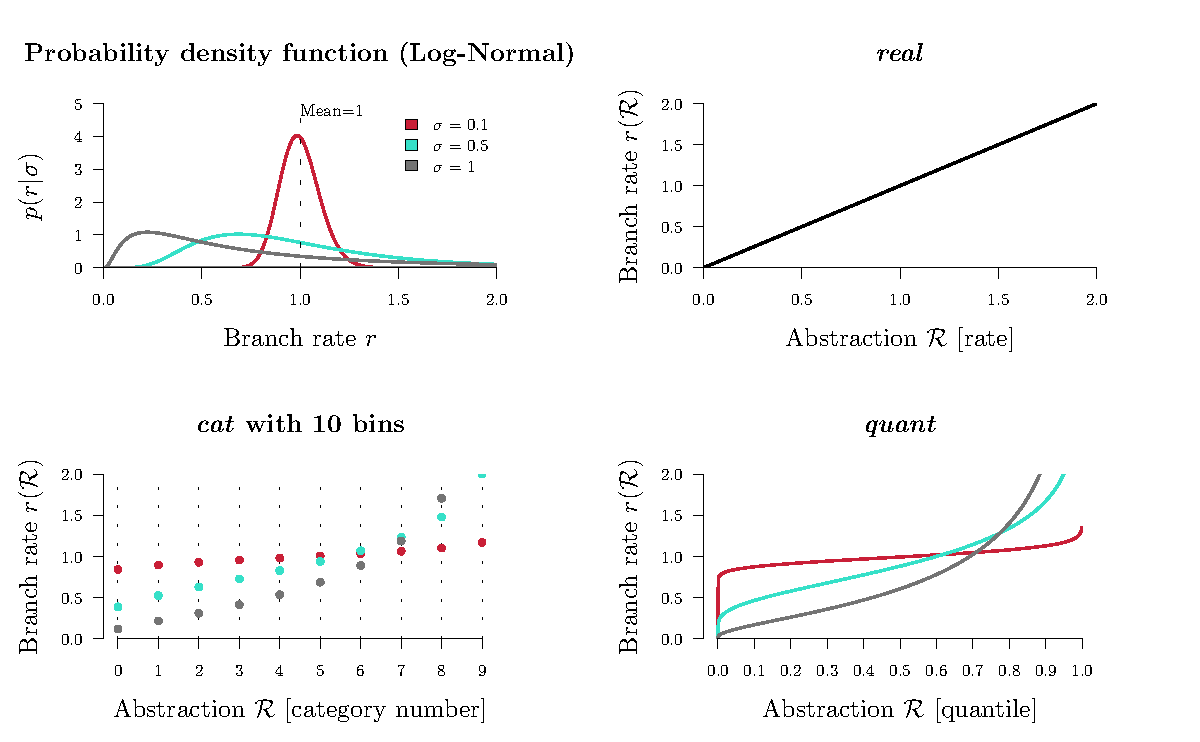
\includegraphics[width=\textwidth]{Figures/rateparameterisation.pdf}
\caption{\textbf{Methods of rate parameterisation.} The \textit{cat} and \textit{quant} approximations are plotted on top of the true underlying rate prior distribution (\textit{real}). In this example, rates are drawn from a $\text{LogNormal}(\mu = -0.045, \sigma = 0.3)$ distribution. The probability density function (pdf) and cumulative density function (cdf) of this distribution are shown.}
\label{fig:rateparams}
\end{figure}




\subsubsection*{1. Real rates}
The natural (and unabstracted) parameterisation of a substitution rate is a real number $\mathcal{R}_i \in \mathbb{R}, \mathcal{R}_i > 0$ which is equal to the rate itself. Thus, under the \textit{real} parameterisation:

% \vec{\mathcal{R}}^{\,} =& \; \vec{r}^{\,} \\
\begin{align}
r(\vec{\mathcal{R}}^{\,}) =& \; \vec{\mathcal{R}}^{\,}.
\end{align}


Under the prior distribution $p(\vec{\mathcal{R}}^{\,} | \sigma)$, rates are often log-normally or exponentially distributed with a mean of 1:

\begin{align}
p(\mathcal{R}_i | \sigma) = \frac{1}{\mathcal{R}_i \sigma \sqrt{2\pi}} \exp \big( -\frac{(\ln \mathcal{R}_i - \mu)^2}{2\sigma^2} \big) \quad &(\text{ LogNormal}(\mu, \sigma)\;) \text{, or}  \\
p(\mathcal{R}_i | \sigma) = p(\mathcal{R}_i) = e^{-\mathcal{R}_i} \quad &(\text{ Exponential}(\lambda=1)\;)
\end{align}


where $\mu = -0.5\sigma^2$ is set such that the expected value of the log-normal distribution is 1.


Zhang and Drummond 2020 present a series of tree operators which propose internal/root node heights, and then recompute the rates of incident branches such that their genetic distances ($r_i \times \tau_i$) remain constant after the proposal. By maintaining genetic distances the likelihood can also be maintained. These operators account for the correlation which exists between branch rates and branch times -- a correlation which is induced by the likelihood function.


%the correlation between rates and times, as imposed by likelihood function, is r after the proposal , and thus lowers the risk of ``falling o

% Such operators are incompatible with the \textit{cat} parameterisation.  The \textit{real} parameterisation and its associated operators yield a mixing rate up to an order of magnitude faster than that of \textit{cat}. \\


\subsubsection*{2. Categories}
The category parameterisation (\textit{cat}) is an abstraction of the \textit{real} parameterisation. Each branch is assigned an integer from $0$ to $n-1$:

\begin{align}
\vec{\mathcal{R}}^{\,} \in& \{ 0, 1, \dotso, n-1 \}^{2N-2}.
\end{align}


The domain of $\vec{\mathcal{R}}^{\,}$ is uniformly distributed:


\begin{align}
p(\mathcal{R}_i | \sigma) = p(\mathcal{R}_i) = \frac{1}{n}.
\end{align}



Let $f(x|\sigma)$ be the probability density function (pdf) and let $F(x|\sigma) = \int\limits_{0}^{x} f(t|\sigma) \; dt$ be the cumulative distribution function (cdf) of the prior distribution used by the underlying \textit{real} clock model. Then, in the \textit{cat} parameterisation, $f(x|\sigma)$ is discretised into $n$ bins and the elements of $\vec{\mathcal{R}}^{\,}$ each point to one of these bins. Each bin contains uniform probability density $1/n$. The rate of each bin is equal to the median value within the bin 


\begin{align}
r(\mathcal{R}_i) =& \; F^{-1}\big(\frac{\mathcal{R}_i + 0.5}{n}\big),
\end{align}

where $F^{-1}$ is the inverse cumulative distribution function (i-cdf).



The key advantage of the \textit{cat} parameterisation is the removal of a term from the posterior density (Equation \ref{eq:bayesian}), or more accurately the replacement of a non-trivial $p(\vec{\mathcal{R}}^{\,} | \sigma)$ term with that of a uniform prior. Thus, one fewer term needs to be estimated per rate.



This method was suggested in the original BEAST2 relaxed clock paper \cite{drummond2006relaxed} and has been widely used. However, the constant distance operators since introduced by Zhang and Drummond 2020 -- which are incompatible with the \textit{cat} parameterisation -- yield an increase in mixing rate under \textit{real} by up to an order of magnitude over that of \textit{cat}.






\subsubsection*{3. Quantiles}


Finally, rates can be parameterised as real numbers $0 < \mathcal{R}_i < 1$ which describe the rate's quantile with respect to some underlying clock model distribution. Under the  \textit{quant} parameterisation, each element in $\vec{\mathcal{R}}^{\,}$ is uniformly distributed.


\begin{align}
\vec{\mathcal{R}}^{\,} \in & \; \mathbb{R}^{2N-2}, 0 < \mathcal{R}_i < 1  \\
p(\mathcal{R}_i | \sigma) = & \; p(\mathcal{R}_i) = 1
\end{align}


Transforming these quantiles into rates invokes the i-cdf of the underlying \textit{real} clock model distribution. Thus, while this approach has clear similarities with \textit{cat}, the domain of rates here is continuous (as opposed to being confined to a discrete number of bins) and is therefore compatible with the class of operators described by Zhang and Drummond 2020. 

A potential disadvantage of the \textit{quant} method would be the computational requirements of continuously evaluating the i-cdf, especially for trees with large $N$. Hence, rather than evaluating the exact i-cdf $F^{-1}$, an approximation $\hat{F}^{-1}$ will be used instead:


\begin{align}
r(\mathcal{R}_i) =& \; \hat{F}^{-1}(\mathcal{R}_i).
\end{align}


In this article we have extended \textit{quant} through a linear piecewise approximation of the i-cdf. As the piecewise approximation is linear, evaluating the derivatives $\frac{\partial}{\partial \mathcal{R}_i} \hat{F}^{-1}(\mathcal{R}_i) =  D \hat{F}^{-1}(\mathcal{R}_i)$ and $\frac{\partial}{\partial r_i} \hat{F}(r_i) = D \hat{F}(r_i)$  -- which are required for computing Hastings ratios -- is trivial. The approximation is comprised of $n$ pieces (where $n$ is fixed) and upper and lower rate boundaries $r_\text{min}$ and $r_\text{max}$. The approximation is displayed in \textbf{Fig \ref{fig:rateparams}} and further detailed in \textbf{\nameref{sect:S1Appendix}}.


Zhang and Drummond 2020 introduced several tree operators for the \textit{real} parameterisation -- including \textbf{Constant Distance}, \textbf{Simple Distance}, and \textbf{Small Pulley}. In this project, we extended these three operators so that they are compatible with the \textit{quant} parameterisation. These are presented in \textbf{\nameref{sect:S1Appendix}}. 



\subsection*{Bactrian proposal kernel} \label{sect:randomwalks}


%The proposal kernel $q(x^\prime|x)$ defines the conditional probability of proposing state $x^\prime$ given state $x$. 

The step size of a proposal kernal $q(x^\prime|x)$ should be such that the proposed state $x^\prime$ is sufficiently far from the current state $x$ to explore vast areas of parameter space, but not so large that the proposal is rejected too often \cite{roberts1997weak}. Yang et al. have challenged the widely used uniform proposal kernel in place of the Bactrian kernel \cite{yang2013searching, thawornwattana2018designing}.
The $\text{Bactrian}(m)$ distribution is defined as the sum of two Normal distributions:


\begin{align}
	\Sigma \sim \text{Bactrian}(m) \equiv \frac{1}{2}\text{Normal}(-m, 1-m^2) + \frac{1}{2}\text{Normal}(m, 1-m^2)
\end{align}


where $0 \leq m < 1$ describes the modality of the Bactrian distribution. When $m=0$, the Bactrian distribution is equivalent to a $\text{Normal}(0, 1)$ distribution. As $m \rightarrow 1$, the distribution becomes increasingly bimodal (\textbf{Fig. \ref{fig:bactrian}}). Yang et al. 2013 \cite{yang2013searching} suggest that $\text{Bactrian}(m=0.95)$ yields a proposal kernel superior to the uniform kernel, by placing minimal probability on steps which are too small or too large.



\begin{figure}[!h]
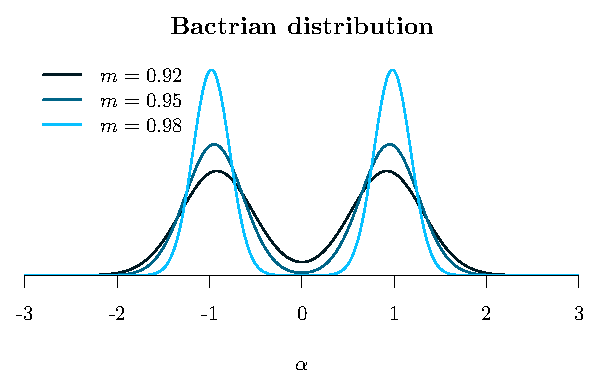
\includegraphics[width=\textwidth]{Figures/bactrian.pdf}
\caption{\textbf{The Bactrian proposal kernel.} Y-axis corresponds to probability density $f(\Sigma|m)$.  }
\label{fig:bactrian}
\end{figure}





In this article we compare the performance of uniform and Bactrian proposal kernels in the clock model. Two Bactrian distributions are compared($m=0.95$ and $m=0.98$). The clock model operators which these proposal kernels apply to are described in \textbf{Table \ref{table:kernels}}.



% Give the equation of the Uniform + Bactrian kernals
% Fig: Bactrian m=0, 0.92, 0.95, 0.98, + Uniform(-1,1)
% In this article we compare the Uniform + Bactrian proposals in the clock model  

% BRIEFLY describe three operators: random walk, scale, uniform + where the proposal kernal comes in + which parameters in the clock model it applies to


\begin{table}[h!]
\centering
\begin{tabular}{|l| l l l|} 
 \hline
 & Operator & Proposal & Parameters  \\
 1 & \textbf{Random walk operator} & $x^\prime \leftarrow x + s\Sigma$ & $\sigma, r, q$ \\
 2 & \textbf{Scale operator} & $x^\prime \leftarrow x \times e^{s\Sigma}$ & $\sigma, r$  \\
 3 & \textbf{Interval operator} & $\begin{array} {rl} y &\leftarrow \frac{u - x}{x - l} \times e^{s\Sigma} \\ x^\prime &\leftarrow \frac{u + l * y}{y + 1}  \end{array}$ & $q \;\; (l=0,u=1)$  \\
 4 & \textbf{Constant distance operators} & $x^\prime \leftarrow x + s\Sigma$ & $t$ \\

 \hline
\end{tabular}
\caption{Summary of proposal kernels $q(x^\prime|x)$ of clock model operators. In each operator, $\Sigma$ is drawn from either a $\text{Bactrian}(m)$ or $\text{Uniform}$ distribution (distributions are normalised so that they have a mean of 0 and a variance of 1). The scale size $s$ is tunable. The proposal kernel may apply to node heights $t$, clock standard deviation $\sigma$, clock rates $r$ (\textit{real} only), and clock rate quantiles $q$ (\textit{quant} only). The Scale operator acts on parameters with non-negative domains. The Interval operator proposes values which respect its domain ie. $l < x^\prime < u$. }
\label{table:kernels}
\end{table}


% $x^\prime \leftarrow w \times \frac{u - x}{x - l}$


\newpage
% REMEMBER to define NNI and SPR acronyms in introduction preferably
\subsection*{Narrow Exchange Rate} \label{sect:NER}

The \textbf{Narrow Exchange} operator \cite{drummond2002estimating}, widely used in BEAST \cite{drummond2012bayesian} and BEAST2 \cite{bouckaert2019beast}, is similar to NNI, and works as follows (\textbf{Fig. \ref{fig:narrowexchange}}):

\textul{\textit{Step 1}}. Sample an internal/root node $E$ from tree $\mathcal{T}$, where $E$ has grandchildren.

\textul{\textit{Step 2}}. Identify the child of $E$ with the greater height. Denote this child as $D$ and its sibling as $C$ (ie. $t_D > t_C$).

\textul{\textit{Step 3}}. Randomly identify the two children of $D$ as $A$ and $B$.

\textul{\textit{Step 4}}. Relocate the $B-D$ branch onto the $C-E$ branch, so that $B$ and $C$ become siblings and their parent is $D$. All node heights are unchanged.


\begin{figure}[!h]
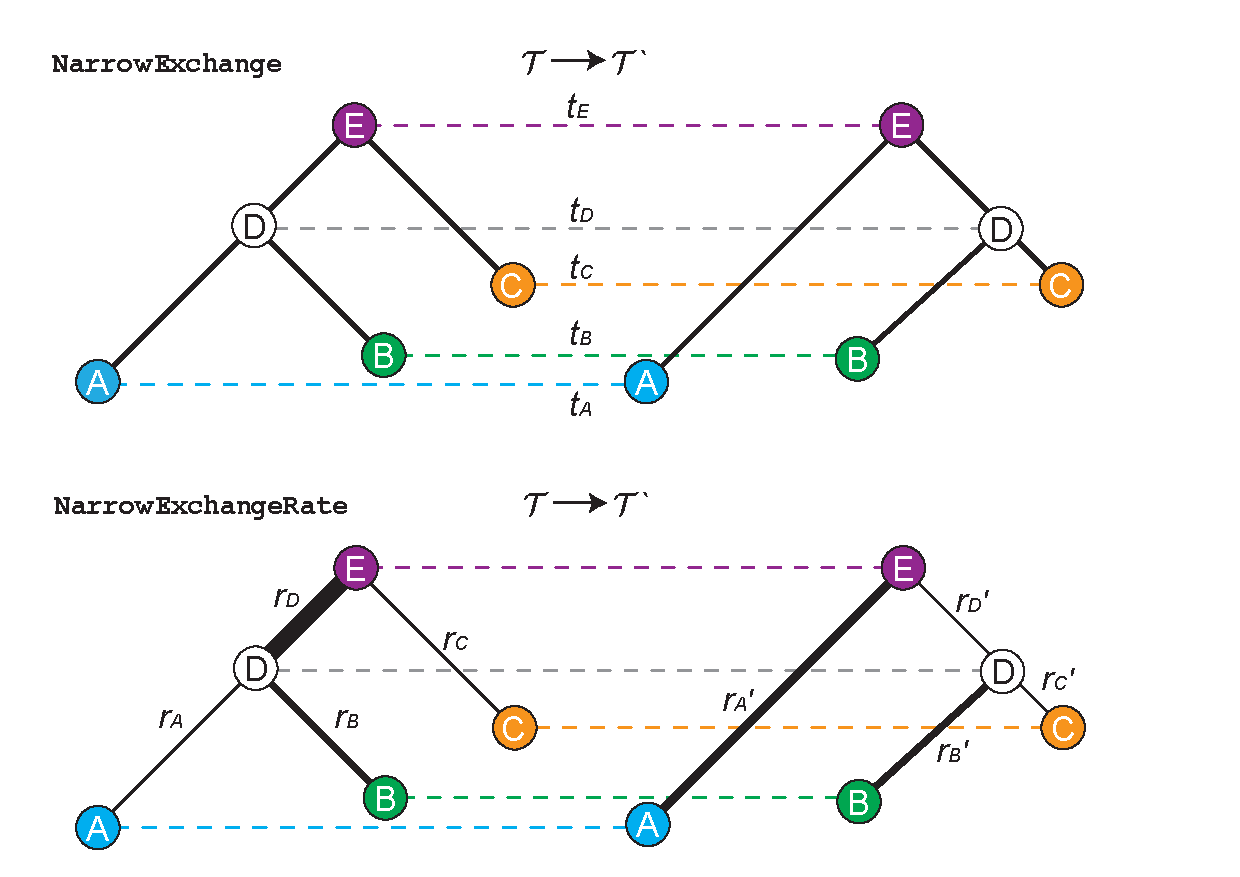
\includegraphics[width=\textwidth]{Figures/NarrowExchange.pdf}
\caption{\textbf{Depiction of Narrow Exchange and Narrow Exchange Rate operators.} Proposals are denoted by $\mathcal{T} \rightarrow \mathcal{T}^\prime$. The vertical axis corresponds to node height $t$. In the bottom figure, branch rates $r$ are indicated by line thickness. In this example, the $\mathcal{D}_{AE}$ and $\mathcal{D}_{CE}$ constraints are satisfied.}
\label{fig:narrowexchange}
\end{figure}


Lakner et al. 2008 \cite{lakner2008efficiency} found that tree operators which perterb topology (such as NNI and SPR) consistently perform better than those which also change branch lengths (such as LOCAL \cite{simon1998local} and Continuous Change \cite{jow2002bayesian}). If Narrow Exchange was adapted to the relaxed clock model by ensuring that genetic distances remain constant after the proposal, its performance may be improved even further. This may in turn permit proposing a new node height $t_D$ and therefore changing branch (time) lengths.

%Therefore, it seems reasonable to adapt the Narrow Exchange operator for use with the relaxed clock model, such that genetic distances remain constant after performing the proposal $\mathcal{T} \rightarrow \mathcal{T}^\prime$.


Here, we present the \textbf{Narrow Exchange Rate} (NER) operator. Let $r_A$, $r_B$, $r_C$, and $r_D$ be the clock rates of nodes $A$, $B$, $C$, and $D$, respectively. In addition to the modest topological change applied by Narrow Exchange, NER also proposes new clock rates ${r_A}^\prime$, ${r_B}^\prime$, ${r_C}^\prime$, and ${r_D}^\prime$. While NER does not alter $t_D$ (ie. ${t_D}^\prime \leftarrow t_D$), we also consider NERw - a special case of the NER operator which embarks $t_D$ on a random walk:

\begin{align}
	{t_D}^\prime \leftarrow t_D + s\Sigma
\end{align}

for random walk step size $s\Sigma$ where $s$ is a tunable scaler parameter and $\Sigma$ is drawn from a uniform or \textbf{\nameref{sect:randomwalks}}. NER (and NERw) are compatible with both the \textit{real} and \textit{quant} parameterisations. Analagous to the Constant Distance operator, new rates are proposed such that genetic distances between nodes $A$, $B$, $C$, and $E$ are maintained. Thus, there are $\binom{4}{2} = 6$ pairwise distance constraints.


\begin{align}
	\mathcal{D}_{AB}: \quad & r_A  (t_D - t_A) + r_B  (t_D - t_B) = \nonumber \\
					 & {r_A}^\prime  (t_E - t_A) + {r_D}^\prime  (t_E - {t_D}^\prime) + {r_B}^\prime ({t_D}^\prime - t_B) \\
	\mathcal{D}_{AC}: \quad & r_A  (t_D - t_A) + r_D  (t_E - t_D) + r_C  (t_E - t_C) = \nonumber \\
				 	  & {r_A}^\prime  (t_E - t_A) + {r_D}^\prime  (t_E - {t_D}^\prime) + {r_C}^\prime ({t_D}^\prime - t_C) \\
 	\mathcal{D}_{AE}: \quad & r_A  (t_D - t_A) + r_D  (t_E - t_D)= \nonumber \\
					  & {r_A}^\prime  (t_E - t_A) \\
  	\mathcal{D}_{BC}: \quad & r_B  (t_D - t_B) + r_D  (t_E - t_D) + r_C  (t_E - t_D)= \nonumber \\
					  & {r_B}^\prime ({t_D}^\prime - t_B) + {r_C}^\prime ({t_D}^\prime - t_C) \\
   	\mathcal{D}_{BE}: \quad & r_B  (t_D - t_B) + r_D  (t_E - t_D)= \nonumber \\
					  & {r_B}^\prime ({t_D}^\prime - t_B) + {r_D}^\prime (t_E - {t_D}^\prime) \\
	\mathcal{D}_{CE}: \quad & r_C  (t_E - t_C)= \nonumber \\
					  & {r_C}^\prime ({t_D}^\prime - t_C) + {r_D}^\prime (t_E - {t_D}^\prime) 
\end{align}


Further constraints are imposed by the model itself:


\begin{align}
	r_i > 0 \text{ and } {r_i}^\prime > 0 \text { for } i \in \{A,B,C,D\} \\
	\max\{t_B, t_C \} < {t_D}^\prime < t_E.
\end{align}



Unfortunately, it is not possible to solve all six $\mathcal{D}_{ij}$ constraints without permitting non-positive rates or illegal trees. Therefore rather than conserving all six pairwise distances, NER conserves a \textit{subset} of distances. It is not immediately clear which distances should be conserved. 


\subsubsection*{Automated generation of operators and constraint satisfaction}


The total space of NER operators is comprised of all possible subsets of distance constraints (ie. $\{\},\{\mathcal{D}_{AB}\}, \{\mathcal{D}_{AC}\}, \dotso , \{\mathcal{D}_{AB}, \mathcal{D}_{AC}, \mathcal{D}_{AE}, \mathcal{D}_{BC}, \mathcal{D}_{BE}, \mathcal{D}_{CE} \}$) which are solvable. The simplest NER -- the null operator denoted by NER$\{\}$ -- does not satisfy any distance constraints. This is equivalent to Narrow Exchange. 

As it is unclear which NER variants would perform the best, we developed an automated pipeline for generating and testing these operators.


\paragraph{1. Solution finding.} Using standard analytical linear-system solving libraries in MATLAB, the $2^6=64$ subsets of distance constraints are solved. 54 out of the 64 subsets were found to be solvable, and the unsolvables were discarded.


\paragraph{2. Solving Jacobian determinants.} The determinant of the Jacobian matrix $J$ is required for computng the Hastings ratio of the proposal. $J$ is defined as 


\begin{align}
	J &= \begin{bmatrix} \frac{\partial {r_A}^\prime}{\partial r_A} & \frac{\partial {r_A}^\prime}{\partial r_B} & \frac{\partial {r_A}^\prime}{\partial r_C} & \frac{\partial {r_A}^\prime}{\partial r_D} \\
	\frac{\partial {r_B}^\prime}{\partial r_A} & \frac{\partial {r_B}^\prime}{\partial r_B} & \frac{\partial {r_B}^\prime}{\partial r_C} & \frac{\partial {r_B}^\prime}{\partial r_D} \\
	\frac{\partial {r_C}^\prime}{\partial r_A} & \frac{\partial {r_C}^\prime}{\partial r_B} & \frac{\partial {r_C}^\prime}{\partial r_C} & \frac{\partial {r_C}^\prime}{\partial r_D} \\
	\frac{\partial {r_D}^\prime}{\partial r_A} & \frac{\partial {r_D}^\prime}{\partial r_B} & \frac{\partial {r_D}^\prime}{\partial r_C} & \frac{\partial {r_D}^\prime}{\partial r_D} \end{bmatrix}.  \nonumber  \\
\end{align}


Computing the determinant $|J|$ invokes standard analytical differentiation and linear algebra libraries of MATLAB. 6 of the 54 operators were found to have $|J|=0$, corresponding to irreversible proposals, and were discarded. 


\paragraph{3. Automated generation of BEAST2 operators.} Java class files are generated using string processing. Each class corresponds to a single operator, extends the class of a meta-NER-operator, and is comprised of the solutions found in \textbf{1} and the Jacobian determinant found in \textbf{2}. $|J|$ is further augmented if the \textit{quant} parameterisation is employed.

The 48 operators generated by this pipeline are evaluated and compared in \textbf{\nameref{sect:results}}. Each operator is considered with and without a random walk on $t_D$ and thus there are 96 total settings.


%Each NER variant differs by its a) proposals, which are the solutions found in step \textbf{1}, and b) its Jacobian $|J|$.  


%On top of topological changes, NER is comprised of proposals for ${r_A}^\prime$, ${r_B}^\prime$, ${r_C}^\prime$, and ${r_D}^\prime$.




\subsection*{Clock model averaging}




\section*{Results and Discussion} \label{sect:results}




\subsection*{Assessment criteria and datasets}


% Cite HKY somewhere hasegawa1985dating


To avoid a cross-product explosion, the three targets for clock model improvement (\textbf{\nameref{sect:rateparams}}, \textbf{\nameref{sect:randomwalks}}, and \textbf{\nameref{sect:NER}}) are evaluated sequentially, in the order presented in this paper. The setting(s) which are considered to be the best in each step are then incorporated into the following step. This protocol and its outcomes are summarised in \textbf{Fig. \ref{fig:tournament}}.

\begin{figure}[!h]
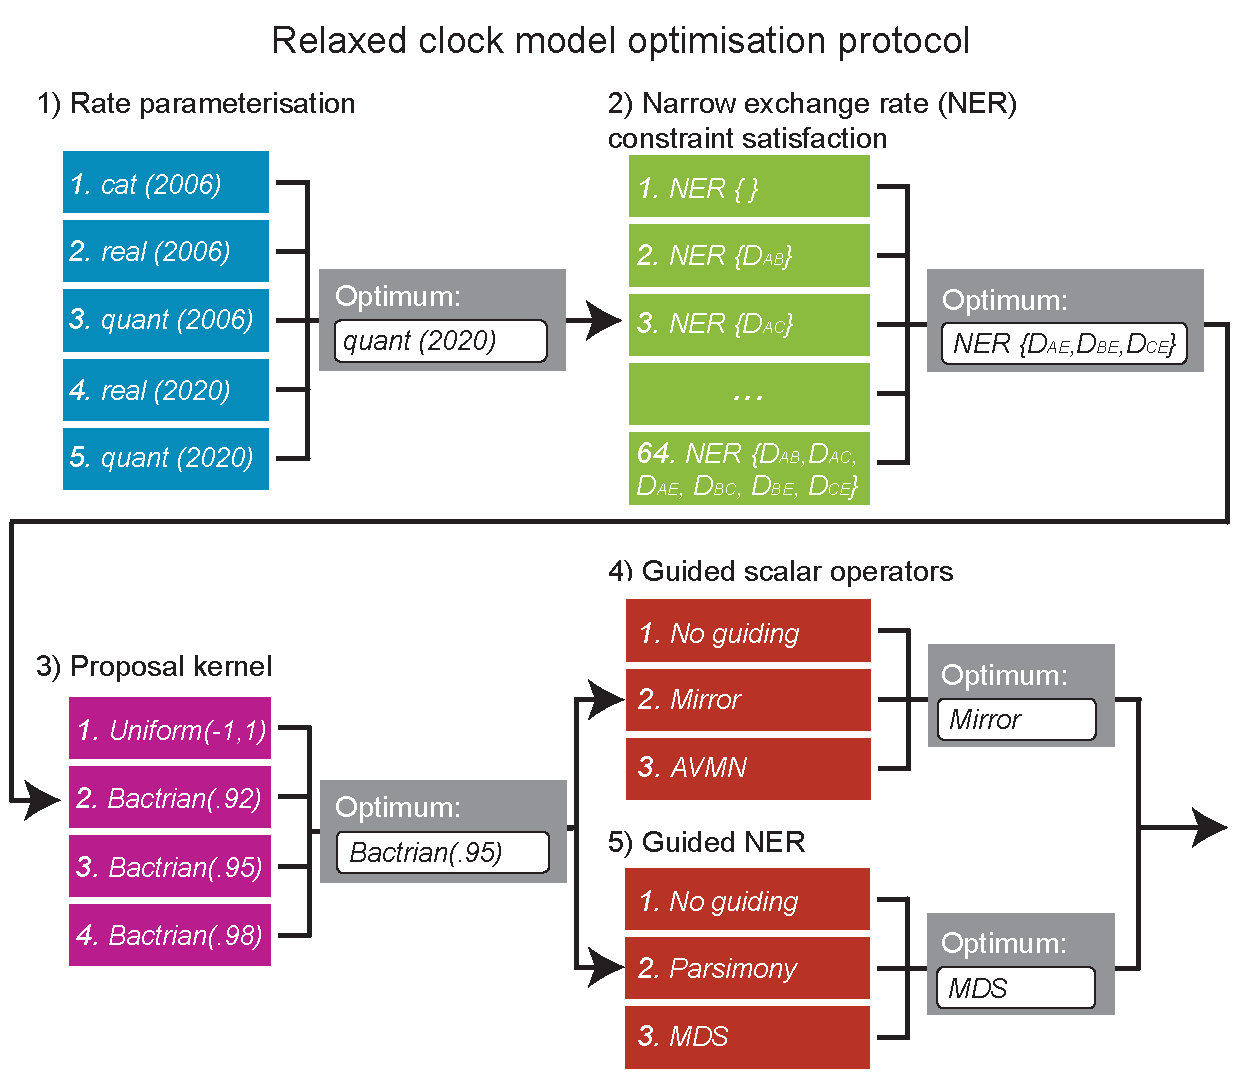
\includegraphics[width=\textwidth]{Figures/tournament.pdf}
\caption{\textbf{Protocol for optimising methodology settings.} The three areas (detailed in \textbf{\nameref{sect:models}}) are optimised sequentially, where the best setting from each step is used when optimising the following step.}
\label{fig:tournament}
\end{figure}


Methodologies are assessed according to the following criteria.


\textbf{1. Validation}. This is assessed by measuring the coverage of all estimated parameters in a well-calibrated simulation study, using 100 simulated datasets (with $N=100$ taxa and $L=5000$ nucleotide alignments). These are presented in \textbf{\nameref{sect:WCSS_appendix}}. \\

\textbf{2. Time to convergence}. Two independent MCMC chains are run and the time is measured until: a) the absolute difference in clade posterior probability between the two chains is less than 0.05 for all clades, b) the Rubin-Gelman statistic $\hat{R}$ \cite{gelman1992inference} of every estimated parameter is less than 1.05, and c) the effective sample size \cite{rambaut2018posterior} of every estimated parameter is greater than 100 in each chain. \\

\textbf{3. Mixing of parameters}. Key parameters are evaluated for the number of effective samples generated per hour (ESS/hr). \\


For the latter two criteria, methodologies are benchmarked using the empirical datasets compiled and partitioned \cite{lanfear2016partitionfinder} by Lanfear \cite{lanfear2019Github}. Four datasets (the spider data by Richart et al. 2015 \cite{Richart_2016}; the turtle data by Crawford et al. 2012 \cite{Crawford_2012}; the caterpillar dataset by Kawahara et al. 2013 \cite{Kawahara_2013}; and the songbird data by Moyle et al. 2016 \cite{Moyle_2016}) are used during the optimisation stage, where each setting is run $10 \times$ and the average statistics across the $10 \times 2 = 20$ chains are reported. All 25 datasets presented in \textbf{Table \ref{table:datasets}} are benchmarked together $1 \times$ each at the end of the protocol. Datasets and BEAST2 .xml templates are provided in the GitHub repository accompanying this article.


Methodologies are benchmarked using the Intel(R) Xeon(R) Gold 6138 CPU (2.00 GHz), with two processing units per pair of MCMC chains.




% https://github.com/roblanf/BenchmarkAlignments
\begin{table}[h!]
\centering
\begin{tabular}{|l| l l l l l|} 
 \hline
  & $N$ & $P$ & $L$ (kb) & $L_\text{eff}$ (kb) & Ref. \\
 
\textbf{1}  &  \textbf{6}  &  1/4/8/\textbf{16}  &  0.4/2.1/10.2/\textbf{13.7}  &  0.1/0.5/1/\textbf{1.1}  &  \textbf{Richart 2015} \cite{Richart_2016} \\ 

\textbf{2}  &  \textbf{10}  &  1/4/8/\textbf{16}  &  0.4/1.5/3.1/\textbf{6.7}  &  0.1/0.3/0.5/\textbf{0.9}  &  \textbf{Crawford 2012} \cite{Crawford_2012} \\ 

3  &  11  &  1/4/8/16  &  0.5/2.2/4.9/10.1  &  0.1/0.4/0.7/1.3  &  Leache 2015 \cite{Leache_2015} \\ 

4  &  18  &  1/4/8/16  &  0.4/1.8/2.9/6.7  &  0.1/0.3/0.4/0.9  &  Meiklejohn 2016 \cite{Meiklejohn_2016} \\ 

5  &  27  &  1/4/8/16  &  0.8/1.4/2/4.3  &  0.3/0.6/1/1.7  &  Faircloth 2013 \cite{Faircloth_2013} \\ 

6  &  33  &  1/4/8/16  &  0.4/1.7/2.6/5.1  &  0.1/0.5/0.7/1.5  &  McCormack 2013 \cite{McCormack_2013} \\ 

7  &  38  &  1/4  &  0.4/2.1  &  0.2/0.6  &  Bergsten 2013 \cite{Bergsten_2013} \\ 

8  &  38  &  1/4/8/16  &  1/2.4/8.1/14.9  &  0.7/1.8/5.6/10.1  &  Ran 2018 \cite{Ran_2018} \\ 

9  &  41  &  1/3  &  0.4/1.7  &  0.3/1.1  &  Brown 2012 \cite{Brown_2012} \\ 

10  &  44  &  1/3  &  0.6/1.9  &  0.2/0.8  &  Cognato 2001 \cite{Cognato_2001} \\ 

11  &  44  &  1/4/7  &  0.8/2.9/5.9  &  0.3/0.8/1.8  &  Dornburg 2012 \cite{Dornburg_2012} \\ 

12  &  51  &  1/4/6  &  0.6/3.5/5.4  &  0.1/0.9/1.8  &  Sauquet 2011 \cite{Sauquet_2011} \\ 

13  &  61  &  1/4/8/16  &  0.9/4.2/7.5/15  &  0.7/2.8/4.6/9.6  &  Broughton 2013 \cite{Broughton_2013} \\ 

14  &  69  &  1/2  &  0.7/0.8  &  0.1/0.1  &  Devitt 2013 \cite{Devitt_2013} \\ 

\textbf{15}  &  \textbf{70}  &  1/\textbf{3}  &  0.7/\textbf{2.2}  &  0.3/\textbf{0.9}  &  \textbf{Kawahara 2013} \cite{Kawahara_2013} \\ 

16  &  78  &  1/4/8/16  &  0.4/1.9/4.1/7.2  &  0.3/1.7/3.6/6.2  &  Cannon 2016 \cite{Cannon_2016} \\ 

17  &  79  &  1/4/8/16  &  0.1/1.3/0.8/4.5  &  0/0.1/0.1/0.8  &  Oaks 2011 \cite{Oaks_2011} \\ 

18  &  94  &  1/4/8/11  &  0.1/1.8/3/3.7  &  0.1/0.8/1.3/1.7  &  Rightmyer 2013 \cite{Rightmyer_2013} \\ 

\textbf{19}  &  \textbf{106}  &  \textbf{1}/4/8/16  &  \textbf{0.6}/3.1/5.1/11.6  &  \textbf{0.3}/1.2/2/4.5  &  \textbf{Moyle 2016} \cite{Moyle_2016} \\ 

20  &  110  &  1/4/8/16  &  0.5/2.1/3.8/7.1  &  0.3/1.4/2.5/4.3  &  Fong 2012 \cite{Fong_2012} \\ 

21  &  152  &  1/4/5  &  1/3.5/3.6  &  0.6/1.6/1.6  &  Day 2013 \cite{Day_2013} \\ 

22  &  187  &  1/4/8/16  &  0.3/0.9/1.4/3.5  &  0.2/0.7/1.1/2.9  &  Branstetter 2017 \cite{Branstetter_2017} \\ 

23  &  197  &  1/4/8/14  &  0.9/3.1/6.1/11.6  &  0.3/1.6/3.5/6.3  &  Horn 2014 \cite{Horn_2014} \\ 

24  &  235  &  1/4/8/16  &  2.3/6.4/8.5/25.7  &  0.9/2.3/3.2/12.2  &  Reddy 2017 \cite{Reddy_2017} \\ 

25  &  237  &  1/4/5  &  0.8/2.4/3.1  &  0.2/1.2/1.5  &  Murray 2013 \cite{Murray_2013} \\ 


 \hline
\end{tabular}
\caption{Empirical datasets used during benchmarking, sorted in increasing order of taxa count $N$. Number of partitions $P$, total alignment length $L$, and number of patterns $L_\text{eff}$ are also specified. Where a dataset is sampled more than once, the dimensions of its multiple samples are separated by `/'. The datasets in bold (Richart 2015 \cite{Richart_2016}, Crawford \cite{Crawford_2012}, Kawahara \cite{Kawahara_2013}, and Moyle \cite{Moyle_2016}) are used during the optimisation protocol. }
\label{table:datasets}
\end{table}






\subsection*{Comparison of rate parameterisations}

We compared the three rate parameterisations described in \textbf{\nameref{sect:rateparams}}. All three settings use the standard BEAST2 clock model operators from Drummond et al. 2006 \cite{drummond2006relaxed}. \textit{real} and \textit{quant} additionally use the constant-distance tree operators described by Zhang and Drummond 2020. To determine whether the difference in performance between \textit{real}/\textit{quant} versus \textit{cat} is because of the constant-distance tree operators or the parameterisation itself, we also included benchmarked two additional settings: \textit{real 2006} and \textit{quant 2006}, which do not used the constant-distance operators. These five settings are validated in \textbf{\nameref{sect:WCSS_appendix}}.


\textbf{Fig. \ref{fig:parameterisationResults}} shows that the \textit{real 2006} performs considerably worse than any of the other settings. This is due to the poor sampling of the prior under this setting (ie. low ESS of $p(\theta)$). The failure of \textit{real 2006} thus highlights the appeal of 1) the \textit{cat} or \textit{quant} parameterisations, both of which have trivial contributions to the prior density (ie. uniform priors), and 2) the smarter operators used by \textit{real} (Zhang and Drummond 2020). Due to its computational burden, \textit{real 2006} was not benchmarked for all of the datasets in \textbf{Table \ref{table:datasets}}.


%Our results are also consistent with Zhang and Drummond 2020, who found that \textit{real} (with constant distance operators) gives superior mixing of rates compared with \textit{cat}. 

Our results show that the \textit{quant} parameterisation yields the best performance with respect to effective samples per hour. \textit{quant} outperforms \textit{quant 2006}, suggesting that the constant distance operators are effective. Furthermore, \textit{quant} outperforms \textit{real} especially at sampling from the posterior and prior distributions (ie. high ESS/hr for $p(\theta|D)$ and $p(\theta)$). This is most likely because of the uniform prior distribution of rate quantiles.

Overall, \textit{quant} yields a median ESS/hr approximately 150 \% faster with respect to sampling the posterior probability, and approximately 30 \% faster with respect to sampling branch rates $r$ and clock standard deviation $\sigma$, compared with \textit{real}.

%\text{cat} and \textit{quant 2006} parameterisations yield similar effective samples per hour for all parameters (including posterior, likelihood, and prior probabilities).  





\begin{figure}[!h]
%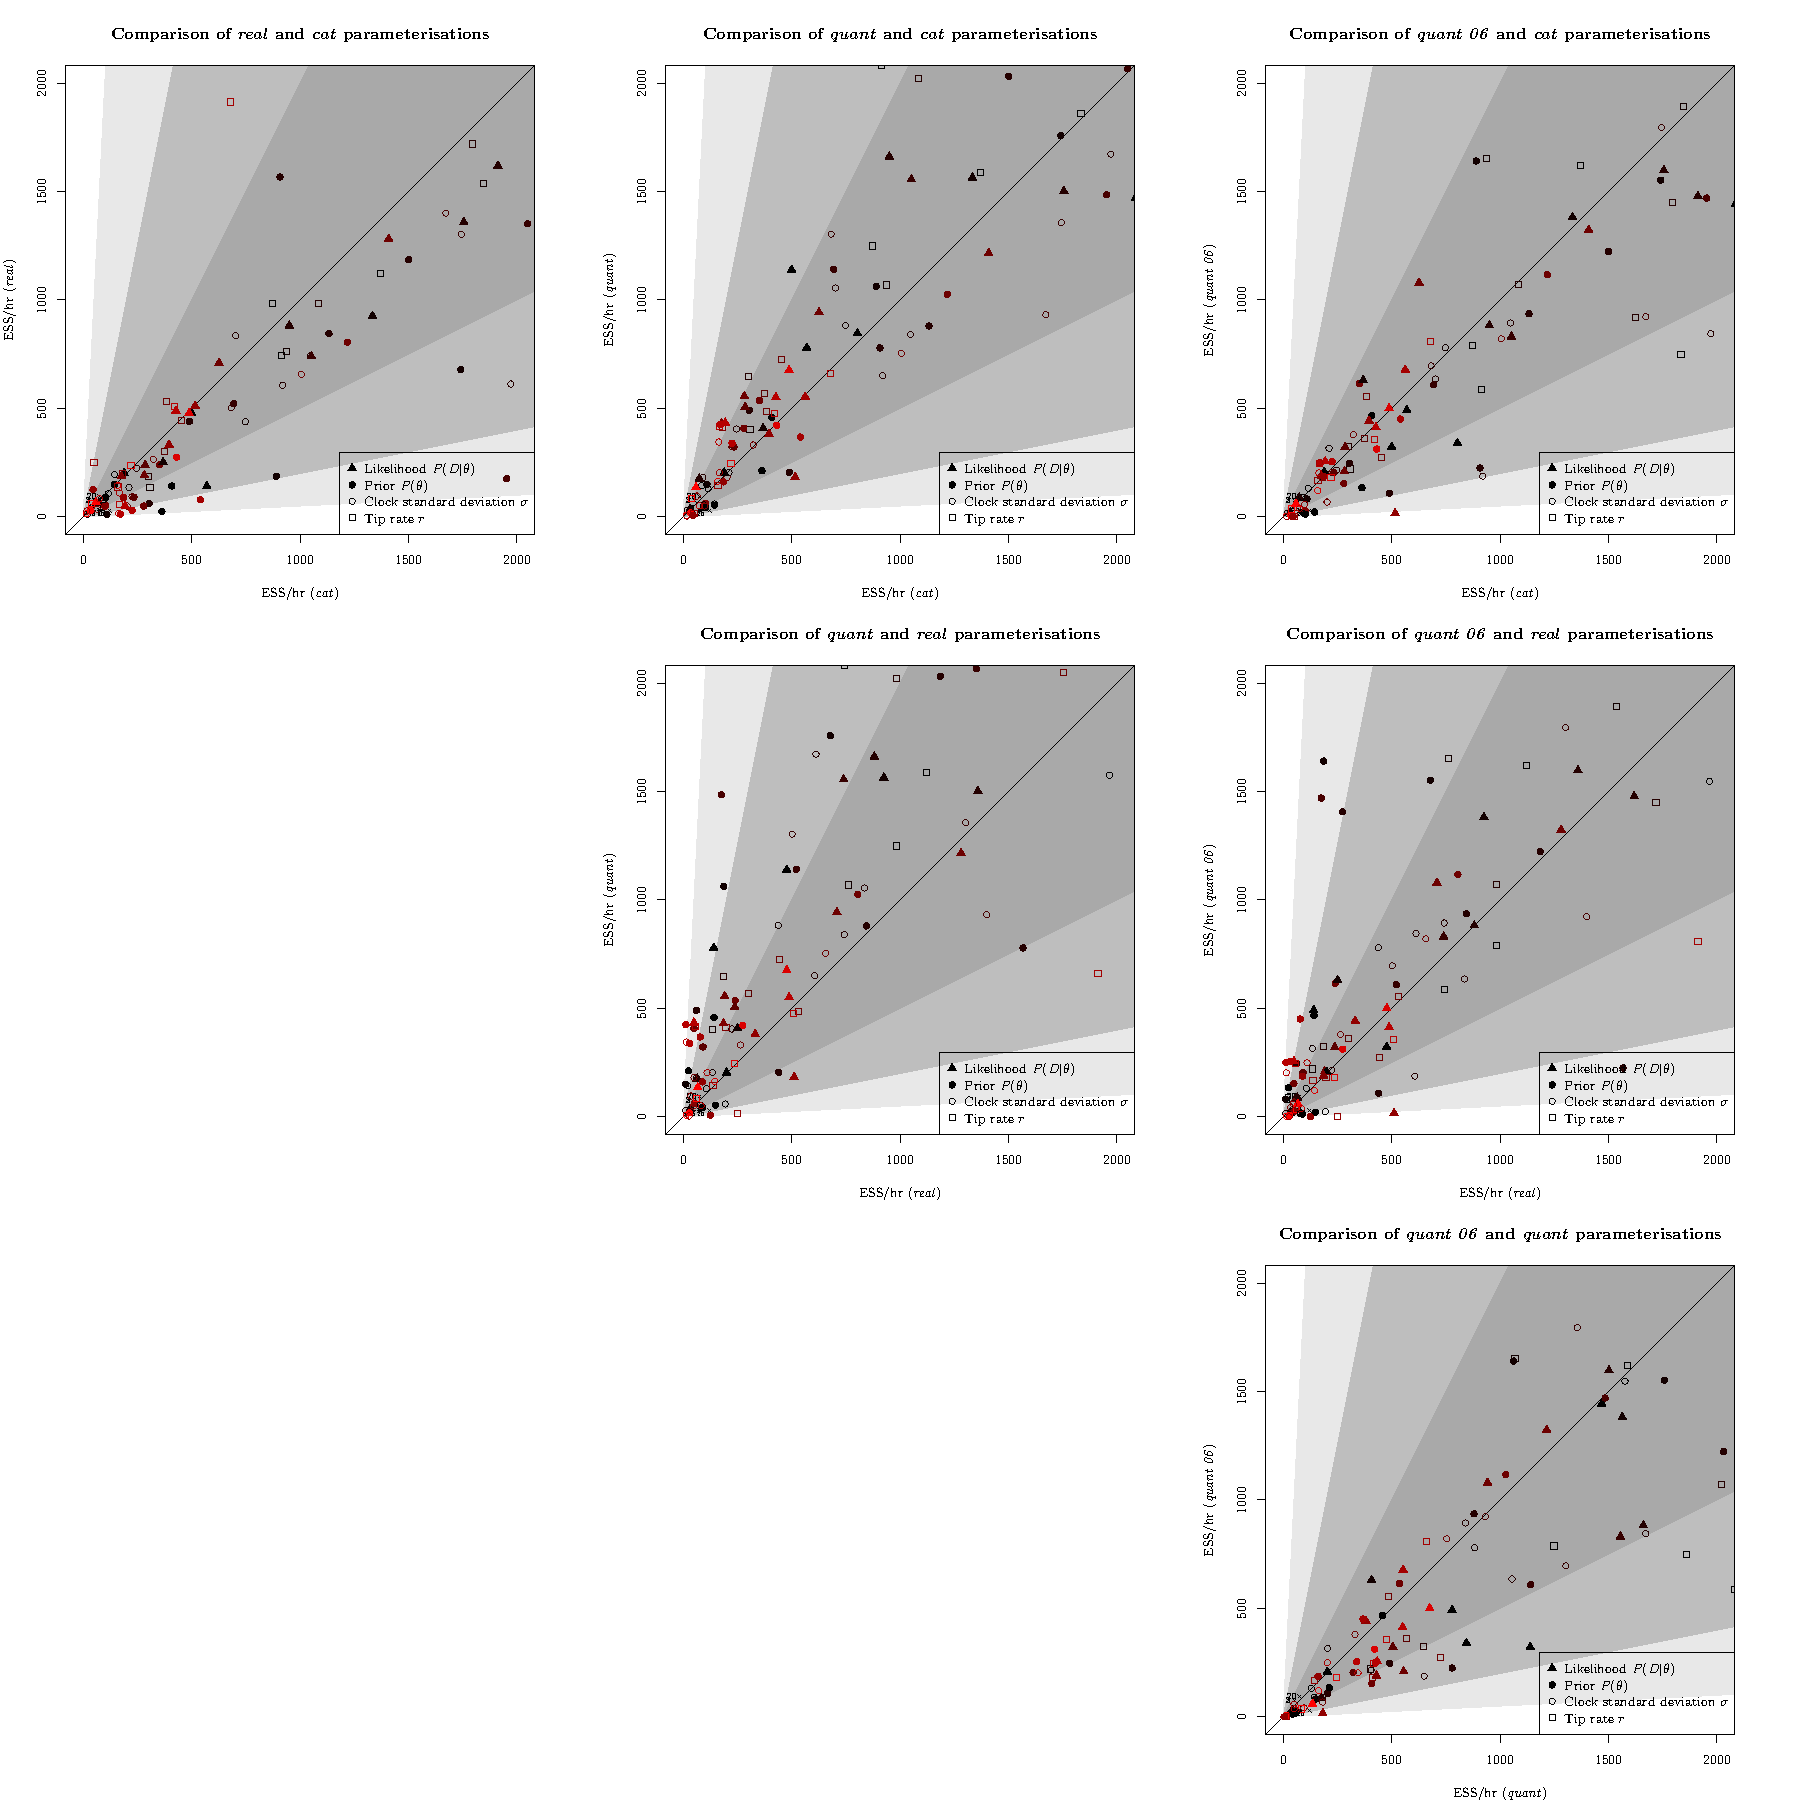
\includegraphics[width=\textwidth]{Figures/ESS.pdf}
\caption{\textbf{Rate parameterisation evaluation.} Comparison of ESS/hr (averaged across two independent MCMC chains) with respect to relevant terms -- $L$: likelihood, $p$: prior density, $r$: clock rate averaged across all leaves, $\sigma$: clock standard deviation. Each point is from one partition sample of the empirical data in \textbf{Table \ref{table:datasets}}.  }
\label{fig:parameterisationResults}
\end{figure}




% 1-3) the \textit{cat}, \textit{real}, and \textit{quant} parameterisations using the operators described by Drummond et al. 2006 \cite{drummond2006relaxed}; 3) the \textit{quant} parameteristion 



\subsection*{Comparison of Bactrian and uniform proposal kernels on the clock model}



\subsection*{Comparison of NER variants}

We compared the Narrrow Exchange Rate (NER) operators described in \textbf{\nameref{sect:NER}}. This protocol selects the best among 48 NER (no random walk) and 48 NERw ($\text{Bactrian}(0.95)$ random walk) operators, and has two phases. First, the best of the 96 is selected by comparing operator acceptance rates on simulated data. Second, the selected operator is benchmarked with respect to convergence time and sampling rate on real data (\textbf{Table \ref{table:datasets}}). All the analyses in this section invoke the \textit{quant} parameterisation and $\text{Bactrian}(0.95)$ proposal kernels on clock model parameters.




\subsubsection*{Initial screening by acceptance rate}


We selected the best operator variant by performing MCMC on 300 simulated datasets, where each MCMC employed all 96 NER/NERw variants. Simulated datasets have $N=30$ taxa and an alignment with $L \sim \text{Uniform}(10^2, 10^4)$ sites. The acceptance rate of each operator is compared to that of the null operator $\text{NER}\{\}$ (ie. Narrow Exchange). 


\textbf{Fig. \ref{fig:acceptanceRateScreening}} shows that NER variants which satisfy the genetic distances between nodes $B$ and $A$ (ie. $\mathcal{D}_{AB}$) or between $B$ and $C$ (ie. $\mathcal{D}_{BC}$) usually perform worse than the standard Narrow Exchange operator, where $B$ is the node being interchanged from the $A$ branch to the $C$ branch (\textbf{Fig. \ref{fig:narrowexchange}}). This is an intuitive result. If the posterior distribution is relatively flat, and the data presents high uncertainty in the positioning of $B$, with respect to $A$ and $C$, then the topological rearrangement performed by Narrow Exchange will be favoured. However, this uncertainty in the \textit{topology} is likely coupled with uncertainty in the \textit{distance} between $B$ and $A$ or between $B$ and $C$. Thus, in this case, respecting the $\mathcal{D}_{AB}$ and $\mathcal{D}_{BC}$ constraints (by proposing branch rates) makes too many unnecessary changes to the state and the operator performs worse.



\begin{figure}[!h]
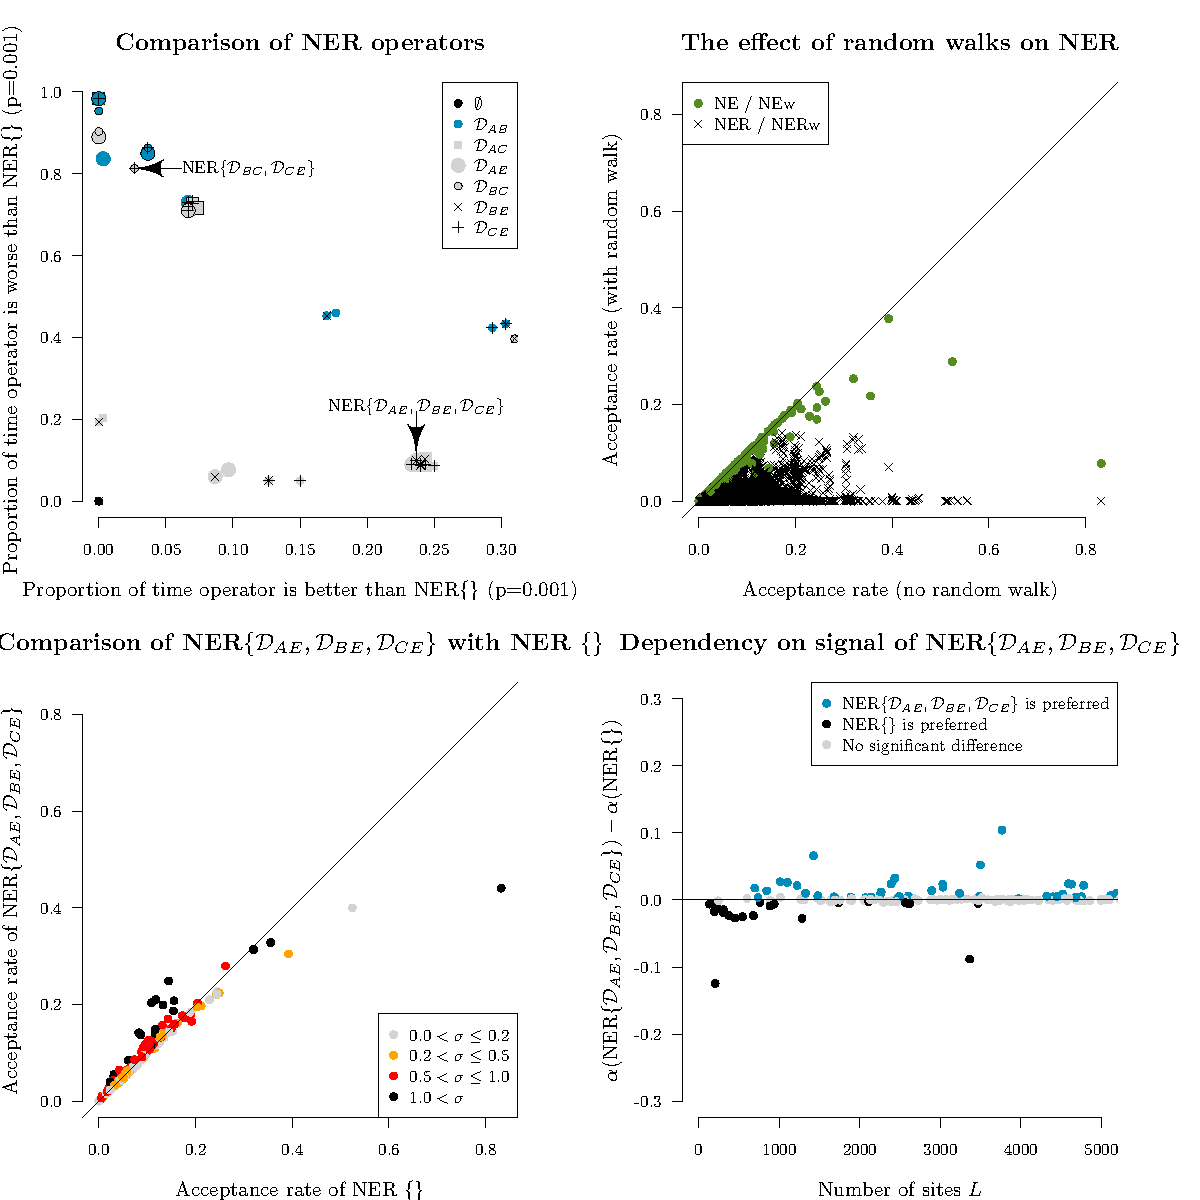
\includegraphics[width=\textwidth]{Figures/acceptanceRates.pdf}
\caption{\textbf{Screening of NER and NERw variants by acceptance rate.} Top left: comparison of NER variants with the null operator $\text{NER}\{\}$ (ie. Narrow Exchange). Each of the 48 operators are represented by a single point, uniquely encoded by the point stylings. The number of times each operator is proposed and accepted is compared with that of $\text{NER}\{\}$, and one-sided z-tests are performed to assess the statistical significance between the two acceptance rates ($p = 0.001$).  This process is repeated for each of $300$ simulated datasets. The axes of each plot are the proportion of these $300$ simulations for which there is evidence that the operator is better than $\text{NER}\{\}$ (x-axis) or worse than $\text{NER}\{\}$ (y-axis). Top right: comparison of NER and NERw acceptance rates. Each point is one NER/NERw variant from a single simulation. Bottom: relationship between the acceptance rates $\alpha$ of $\text{NER}\{\mathcal{D}_{AE}, \mathcal{D}_{BE}, \mathcal{D}_{CE}\}$ and $\text{NER}\{ \}$ with the clock model standard deviation $\sigma$ and the number of patterns $L_\textit{eff}$.  Each point is a single simulation. }
\label{fig:acceptanceRateScreening}
\end{figure}





\textbf{Fig. \ref{fig:acceptanceRateScreening}} also reveals a cluster of NER variants which -- under the conditions of the simulation --  performed better than the null operator $\text{NER}\{\}$ around 25\% of the time and performed worse around 10\% of the time. One such operator is  $\text{NER}\{\mathcal{D}_{AE}, \mathcal{D}_{BE}, \mathcal{D}_{CE}\}$. This variant conserves the genetic distance between all child nodes $A$, $B$, and $C$, and the grandparent node $E$. This is performed by proposing rates for $r_A$, $r_B$, and $r_C$ while obeying the distance constraints imposed by the operator. Exploring this operator further, we can see that $\text{NER}\{\mathcal{D}_{AE}, \mathcal{D}_{BE}, \mathcal{D}_{CE}\}$ is at its best when there is a large variance in branch rate ie. when clock standard deviation $\sigma$ is high ($\sigma \gtrsim 0.5$ for $N=30$), corresponding to data which is not clock-like. On the other hand, $\text{NER}\{\}$ is much preferred when the operator's acceptance rate is high ($\gtrsim 0.15$) -- corresponding with datasets with a small number of site patterns ($L_\textit{eff} \lesssim 500$ for $N=30$) and thus poor signal.  Overall, $\text{NER}\{\mathcal{D}_{AE}, \mathcal{D}_{BE}, \mathcal{D}_{CE}\}$ outperforms the standard Narrow Exchange operator when the data is not clock-like and contains enough signal. 




Finally, \textbf{Fig. \ref{fig:acceptanceRateScreening}} shows that by applying a (Bactrian) random walk to $t_D$ -- the height of internal node $D$ -- the acceptance rate of NER plummets dramatically. This effect is most dominant for the NER variants which satisfy distance constraints (ie. the operators which are not $\text{NER}\{\}$). This result is unfortunate however not unexpected, and is consistent with Lakner et al. 2008 \cite{lakner2008efficiency}, who observed that tree operators perform best when they change either topology, or branch lengths, but not both.



Although there are several operators tying for first place, we selected the $\text{NER}\{\mathcal{D}_{AE}, \mathcal{D}_{BE}, \mathcal{D}_{CE}\}$ operator to proceed to the next round of optimisation.





\subsubsection*{Benchmarking convergence time}





\section*{Conclusion}


\newpage
\section*{Supporting information}


\paragraph*{S1 Appendix.}
\label{sect:S1Appendix}
{\textbf{Rate quantiles.} The linear piecewise approximation used in the \textit{quant} parameterisation is described. Tree operators presented by Zhang and Drummond 2020 are extended to the \textit{quant} parameterisation. 



\paragraph*{S2 Appendix.}
\label{sect:WCSS_appendix}
{\textbf{Well-calibated simulation studies.} Methodologies are validated using well-calibated simulation studies.




\nolinenumbers

% Either type in your references using
% \begin{thebibliography}{}
% \bibitem{}
% Text
% \end{thebibliography}
%
% or
%
% Compile your BiBTeX database using our plos2015.bst
% style file and paste the contents of your .bbl file
% here. See http://journals.plos.org/plosone/s/latex for
% step-by-step instructions.
%

\newpage
\bibliography{references}



\end{document}












